\clearpage
\section{Error analysis}\label{app:errors}
There is one figure per dataset (\cref{app:errors-unsw,app:errors-ton,app:errors-bot,app:errors-cic,app:errors-edge}).
In each figure, the top panel shows the per-class F1 of every method (mean over seeds). The bottom panel shows
confusion matrices for XGBoost and for the best encoding of each language model, as the share of each true class.

\subsection{NF-UNSW-NB15}\label{app:errors-unsw}
\begin{figure}[H]
  \centering
  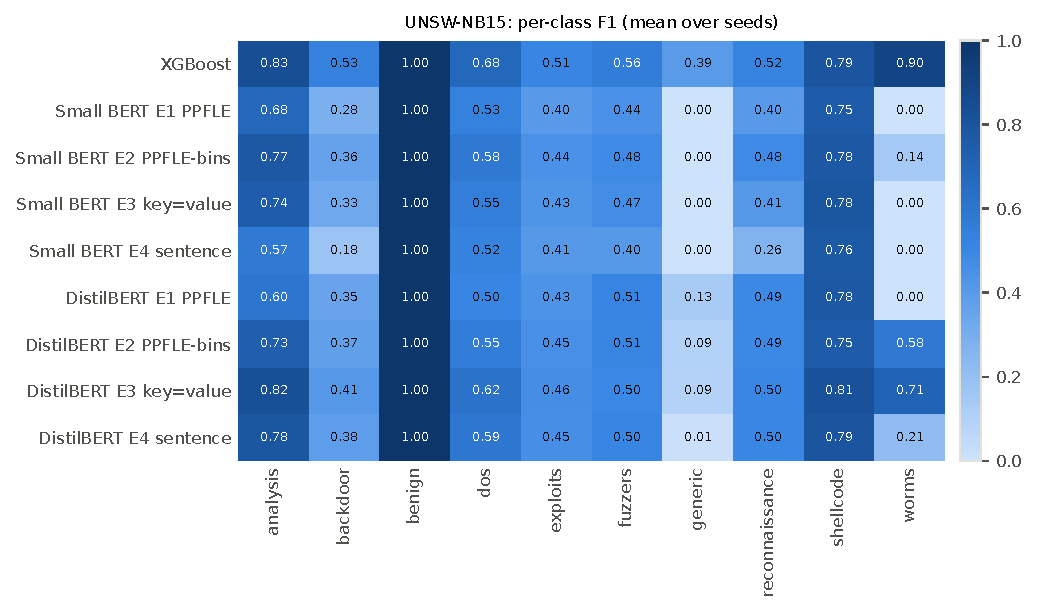
\includegraphics[width=\linewidth]{perclass_f1_nf_unsw_nb15}
  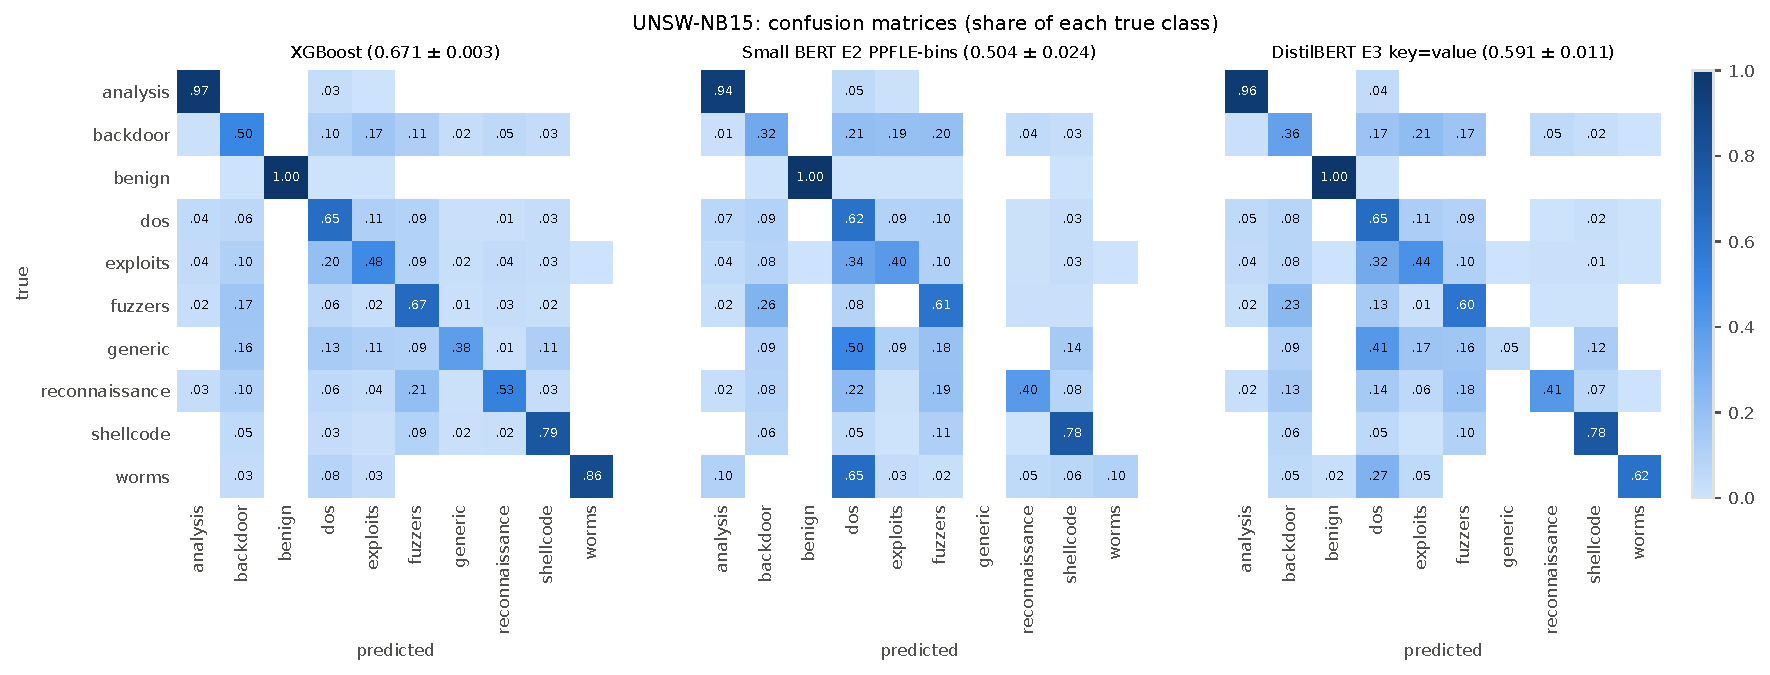
\includegraphics[width=\linewidth]{confusion_nf_unsw_nb15}
  \caption{Appendix C. Error analysis, NF-UNSW-NB15: per-class F1 (top) and confusion matrices (bottom).}
\end{figure}

\subsection{NF-ToN-IoT}\label{app:errors-ton}
\begin{figure}[H]
  \centering
  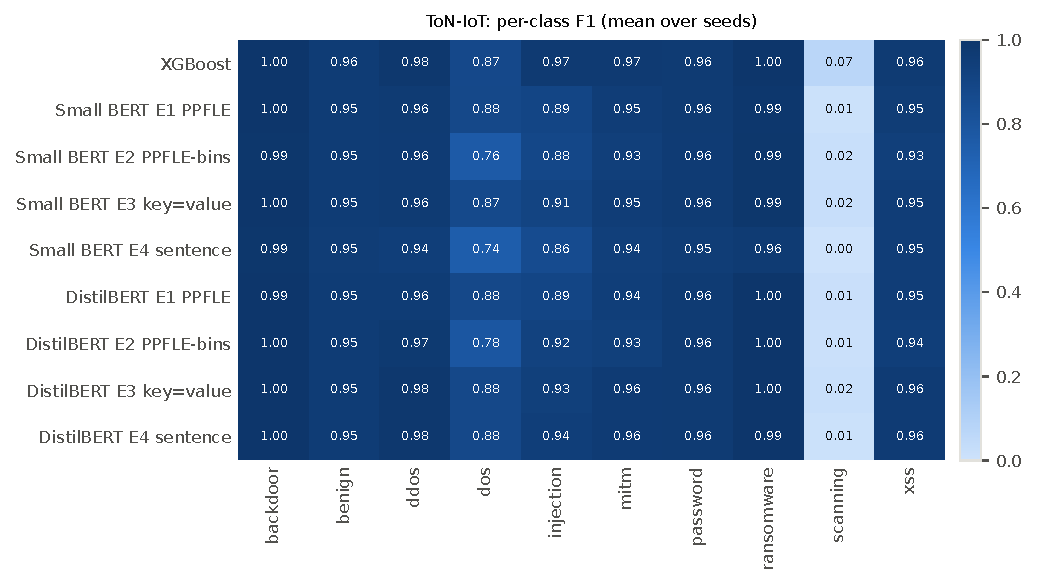
\includegraphics[width=\linewidth]{perclass_f1_nf_ton_iot}
  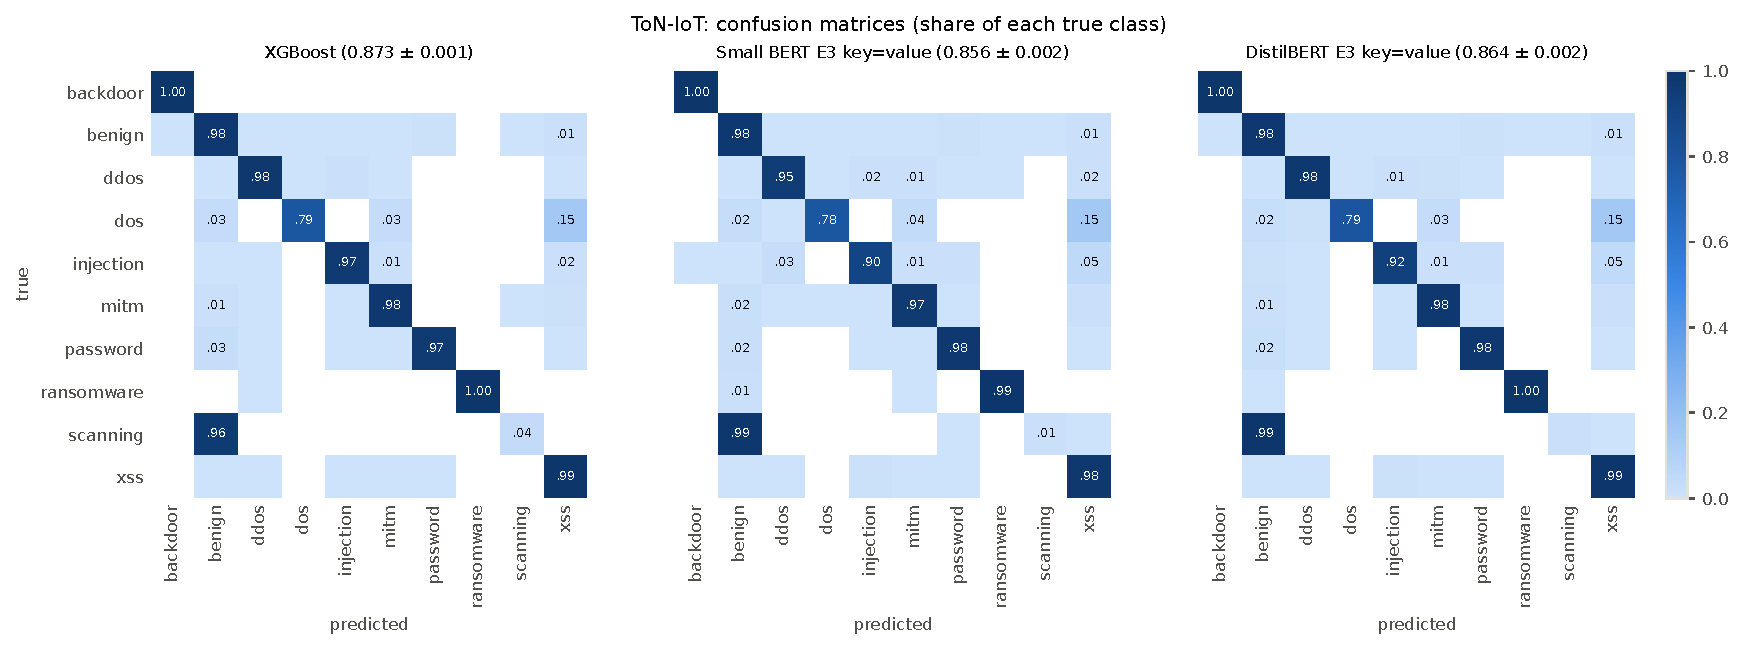
\includegraphics[width=\linewidth]{confusion_nf_ton_iot}
  \caption{Appendix C. Error analysis, NF-ToN-IoT: per-class F1 (top) and confusion matrices (bottom).}
\end{figure}

\subsection{NF-BoT-IoT}\label{app:errors-bot}
\begin{figure}[H]
  \centering
  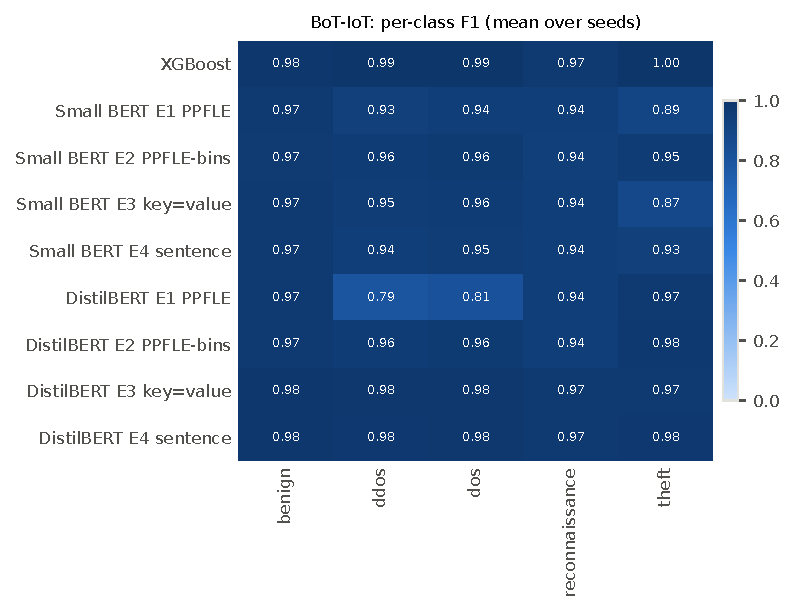
\includegraphics[width=\linewidth]{perclass_f1_nf_bot_iot}
  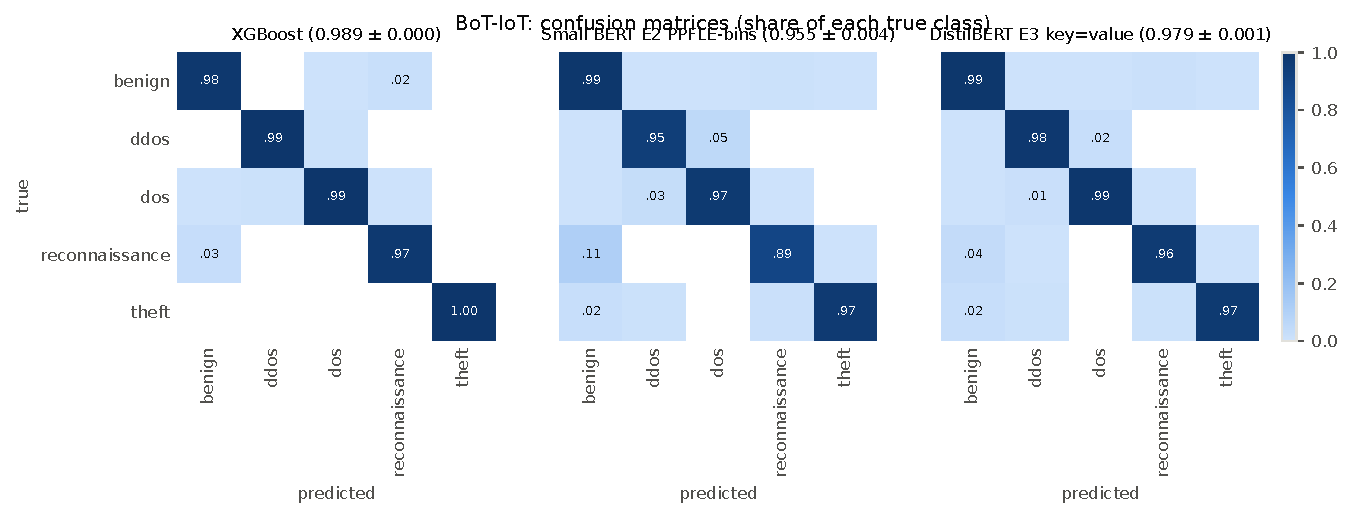
\includegraphics[width=\linewidth]{confusion_nf_bot_iot}
  \caption{Appendix C. Error analysis, NF-BoT-IoT: per-class F1 (top) and confusion matrices (bottom).}
\end{figure}

\subsection{NF-CSE-CIC-IDS2018}\label{app:errors-cic}
\begin{figure}[H]
  \centering
  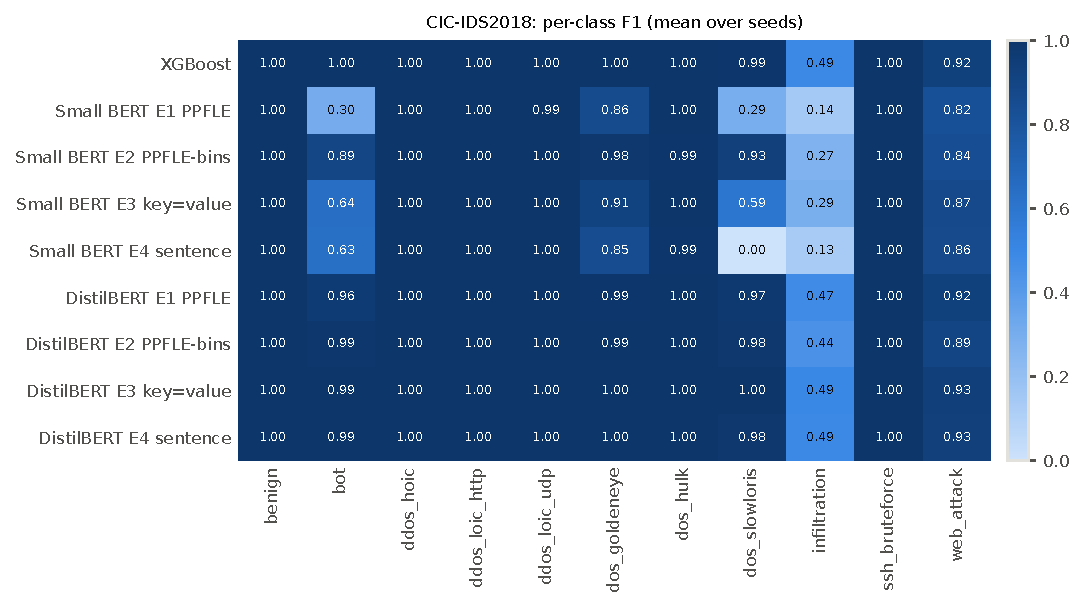
\includegraphics[width=\linewidth]{perclass_f1_nf_cse_cic_ids2018}
  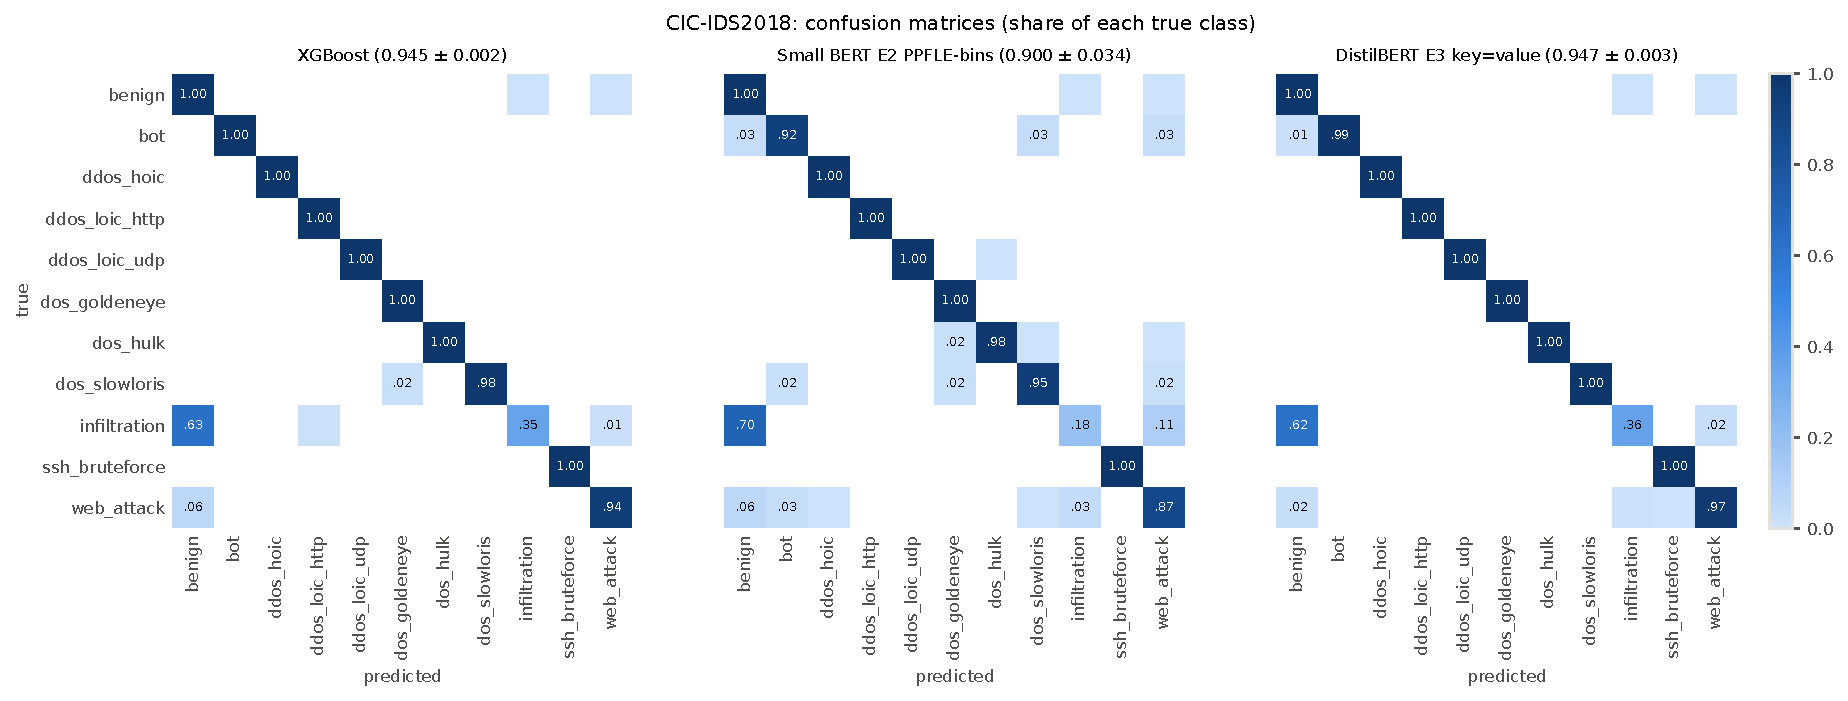
\includegraphics[width=\linewidth]{confusion_nf_cse_cic_ids2018}
  \caption{Appendix C. Error analysis, NF-CSE-CIC-IDS2018: per-class F1 (top) and confusion matrices (bottom).}
\end{figure}

\subsection{Edge-IIoTset}\label{app:errors-edge}
\begin{figure}[H]
  \centering
  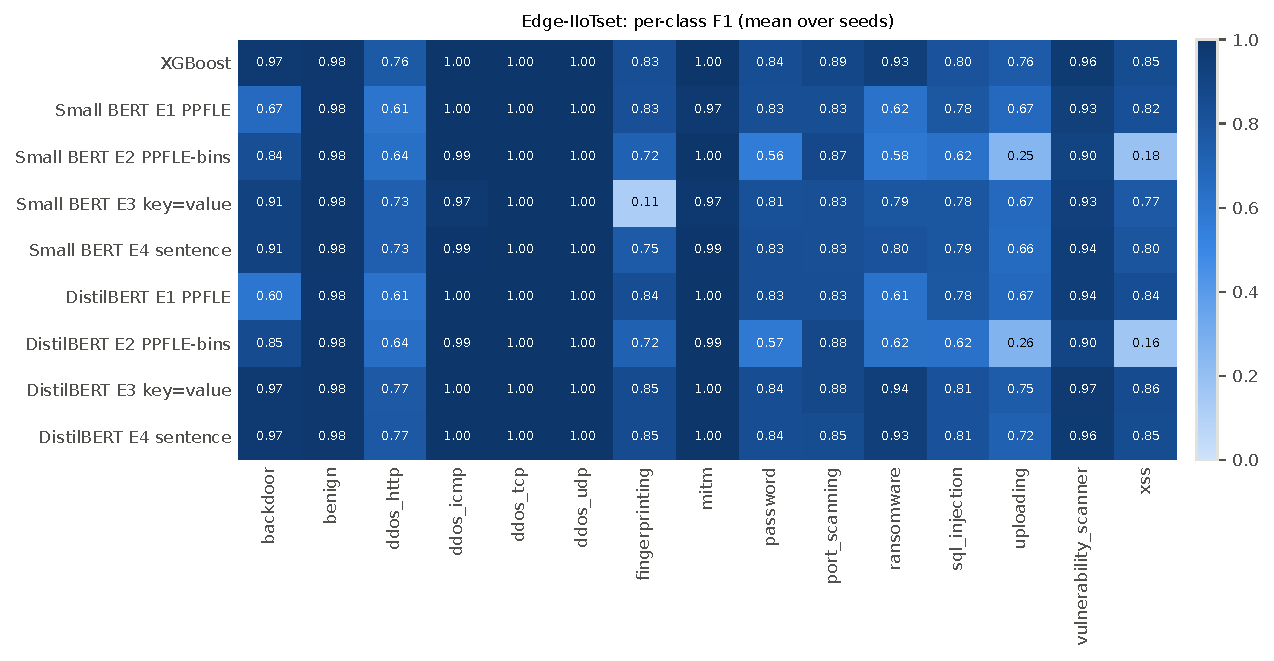
\includegraphics[width=\linewidth]{perclass_f1_edge_iiotset}
  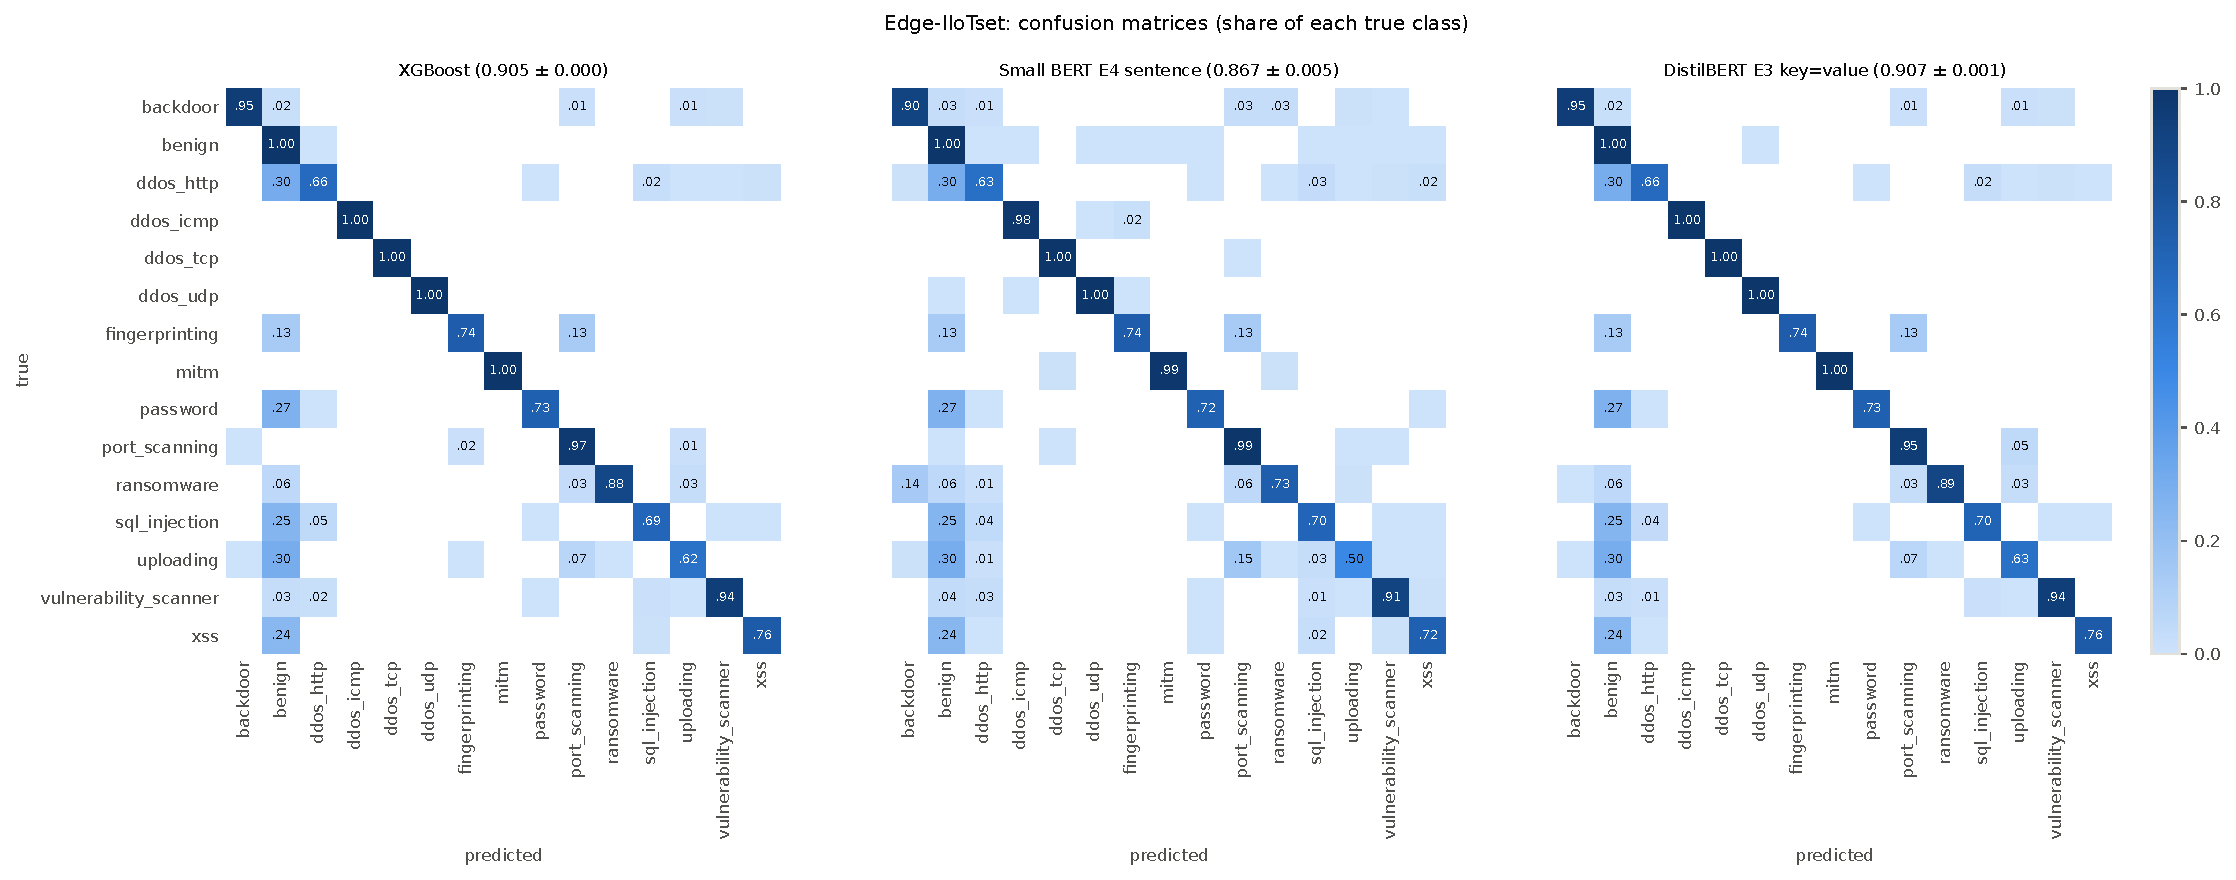
\includegraphics[width=\linewidth]{confusion_edge_iiotset}
  \caption{Appendix C. Error analysis, Edge-IIoTset (fixed data): per-class F1 (top) and confusion matrices (bottom).}
\end{figure}
